\chapter{Data}

Because there is intrinsic variability in the number of near-Earth objects colliding with Earth's atmosphere from night-to-night, a sufficient data sample plays a vital role in estimating an average flux.
This chapter details our data sample, specifically with respect to our time, observable area, and fireball distributions.  
To assess the overall capabilities of our system, we also delve into the data behind our star catalog, previously used for total observable area calculations.  
While this chapter provides the raw data samples and overall distributions, a further analysis and interpretation of the data can be found in Chapter 5.

\section{Time Distributions}

The D6 AllSky Camera does have a protective shell, however it is not always placed outside for nightly observations.
Due to Oregon's climate, we often leave our observation system inside.
There have been a total of $221$ days between August 27, 2018, the beginning of Willamette's academic year, and May 6, 2019.
Out of those $221$ days, we have been able to observe for \hl{$34$} nights, for a total of \hl{$291.87$} hours.

Once placed outside to observe, the D6 AllSky Camera begins taking observation when the sky is dark enough to take videos of without fear of over-saturation.
As the sky gets brighter when sunrise approaches, the camera automatically shuts off, ending the observation session.
This brightness constraint means that the total observation time changes from night-to-night.
We observed for an average of \hl{$8.584$} hours per night.
The shortest observation session lasted \hl{$7$} hours while the longest lasted \hl{$11$} hours.


\begin{figure}[ht!]
  \centering
  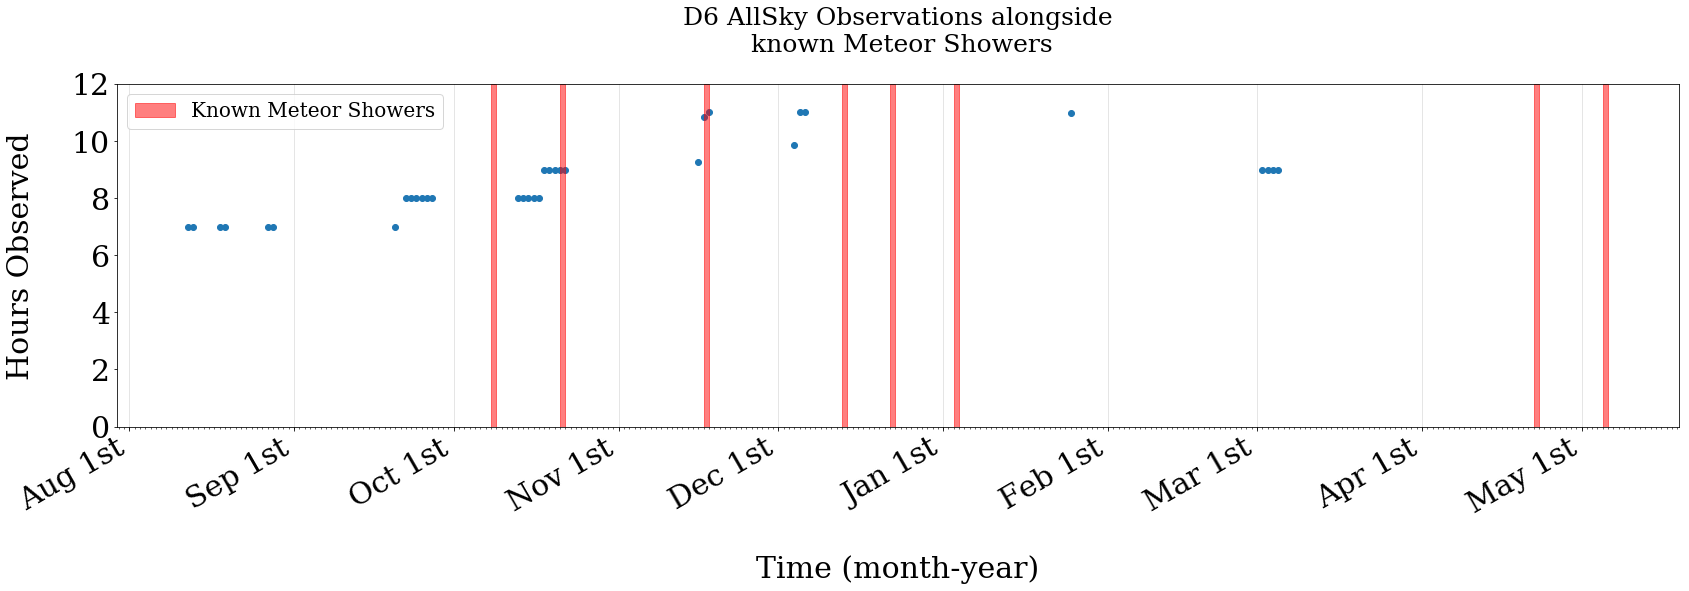
\includegraphics[scale=0.25]{images/nights_observed_with_meteorshowers.png}
  \caption{A plot of all D6 AllSky observation dates and recognized meteor showers within the $2018-2019$ academic calendar year.}
  \label{dateplot}
\end{figure}


Figure \ref{dateplot} displays the individual nights that we observed throughout the academic calendar. 
In addition to plotting our observation dates and that sessions total observing time, we have indicated dates of meteor showers visible in Salem, Oregon.  
During the months of October and November, we observed on nights of the Orionid and Leonid showers respectively.  
% Insert smooth transition




\section{Coverage Distributions}

As described in the methodology section, to calculate the angular distance per pixel for a given location, we needed two different celestial object measurements.
By taking the angular separation between the two, we designated the ratio to their respective midpoint.  
In total, we used \hl{$2638$} comparisons to create our angular separation per pixel data-set.  
Figure \ref{angperpix1} shows all of these points, each colored with their respective angular separation per pixel ratio.  

\begin{figure}[ht!]
  \centering
  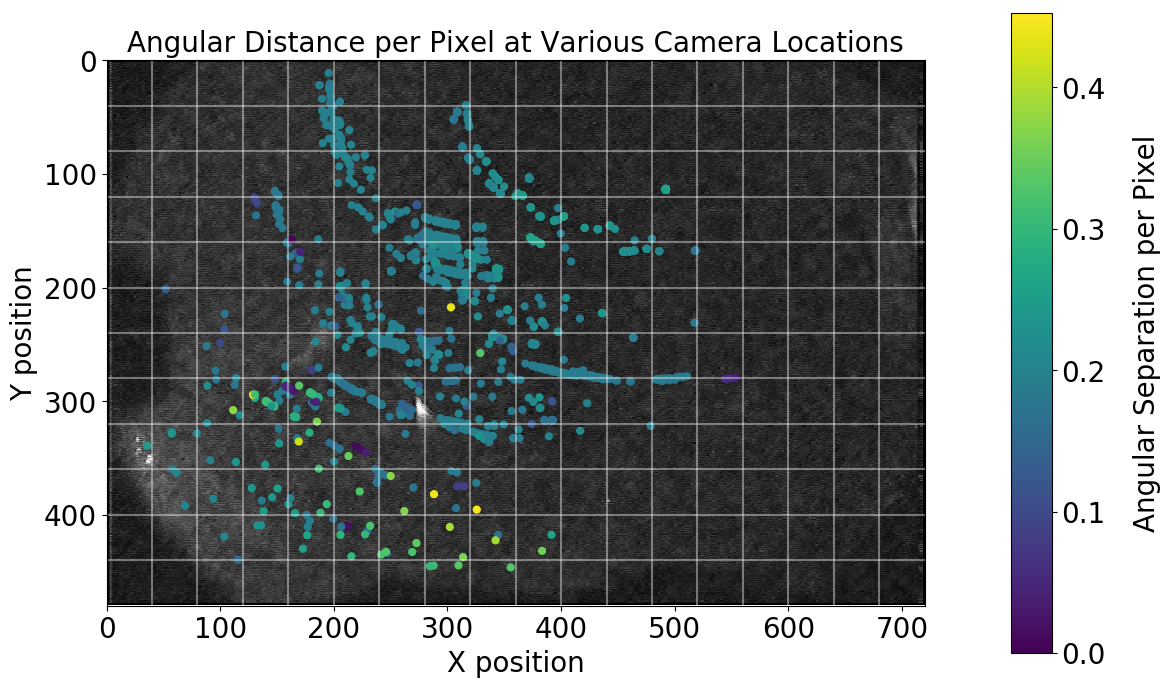
\includegraphics[scale=0.4]{images/angular_distance_at_various_locations.png}
  \caption{A plot of angular separation per pixel measurements from celestial comparisons.}
  \label{angperpix1}
\end{figure}

One may note that Fig. \ref{angperpix1} shows many data points, but they do not span the entirety of the camera field. 
There are many regions with no data points.
Because has a view that is symmetric about the azimuth, we rotated all of our data points by a fixed quantity and appended them to the current data set.  
This assumption of azimuthal symmetry allowed us to attain a more robust data sample without sacrificing data quality.
By rotating and appending in sequences of $5\degree$ in a full unit circle, we were able to increase the number of data points by a magnitude of \hl{$71.53$}.
From this point we were able to then bin the data and create Fig. \ref{colorful}.


\begin{figure}[ht!]
  \centering
  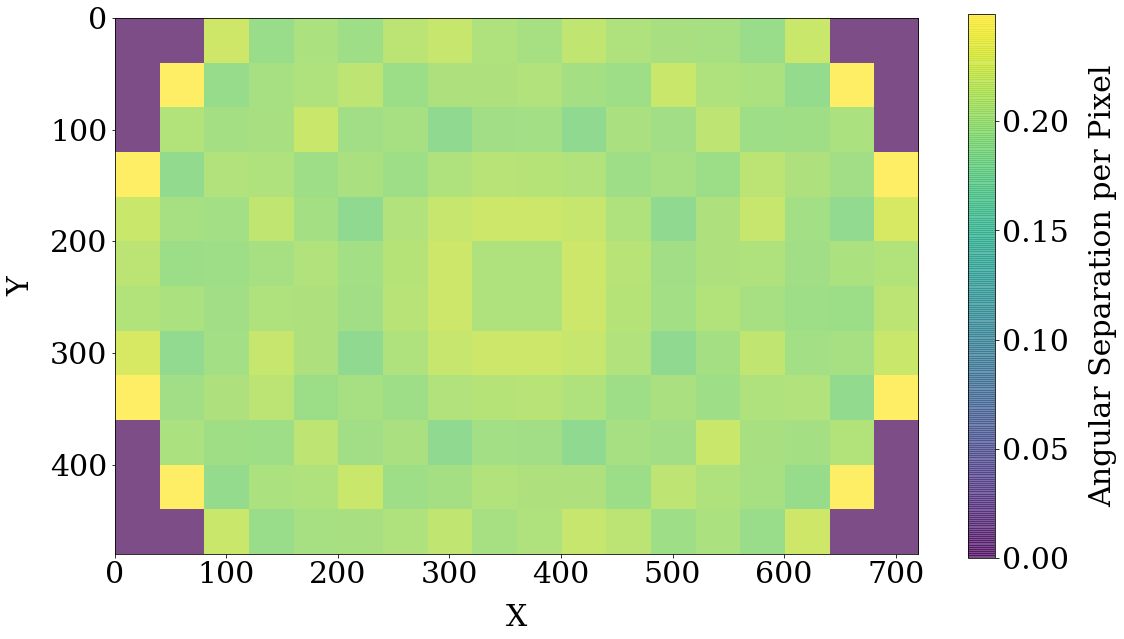
\includegraphics[scale=0.35]{images/boxes_colored.png}
  \caption{Average angular separation per pixel for different camera pixel regions.}
  \label{colorful}
\end{figure}

As described in the Background chapter, we used our measured solid angles for each region to calculate individual rectangular pyramid-created sky areas at a fixed radius of \SI{11.4}{k\meter}
Our measured total areal coverage was \hl{$->$} \SI{58974.88}{k\meter}$^2$ \hl{$<-$}.

As some nights were cloudy and others clear, the observable area value fluctuated in time. 
Figure \ref{time_area} depicts both the total observation time and the average observable area for each of our observation months. 

\begin{figure}[ht!]
  \centering
  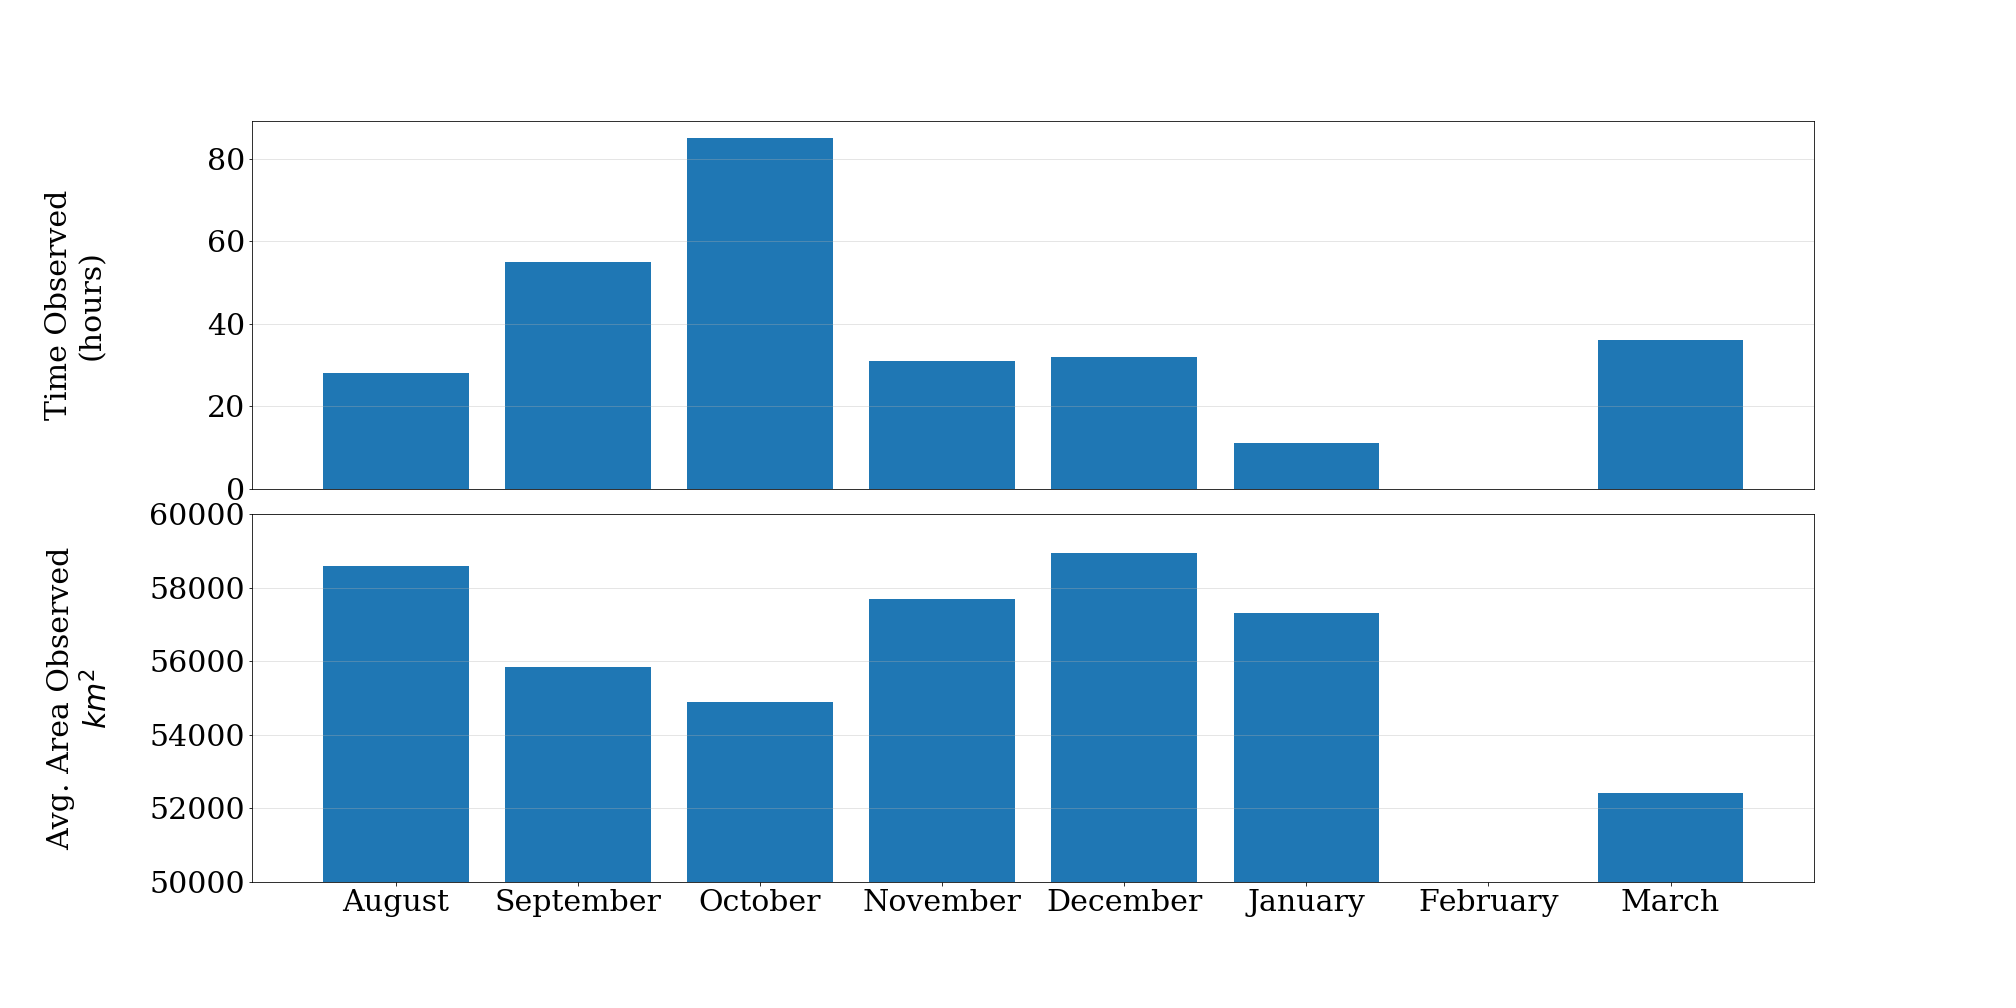
\includegraphics[scale=0.25]{images/time_vs_areaobs_plot.png}
  \caption{A plot of total observation time and average observable area for each month.}
  \label{time_area}
\end{figure}

Our average observable area across all observations was \hl{$->$} \SI{56012.03}{k\meter}$^2$ \hl{$<-$}.
This value, along with our total observation time and number of events will be used to determine the overall average flux.
% Insert smoother transition than this ^


\section{Detected Fireballs}

In total, the D6 AllSky Camera captured a total of \hl{$1095$} videos.  
Of those \hl{$1095$}, only \hl{$6$} were identified as real fireballs.
A depiction of the locations of these fireballs can be found in Fig. \ref{fireball_locs}.  

\begin{figure}[ht!]
  \centering
  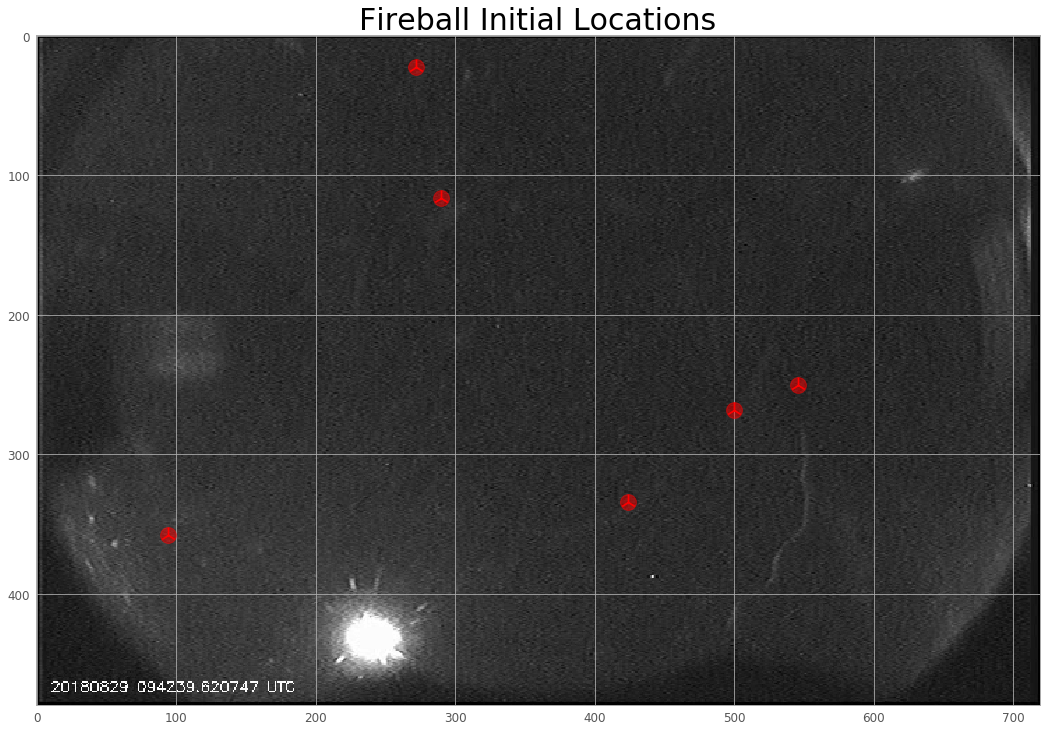
\includegraphics[scale=0.25]{images/fireball_initlocs.png}
  \caption{The initial pixel locations of all detected fireballs.}
  \label{fireball_locs}
\end{figure}

Of the \hl{$6$} fireballs, $3$ were found within $24$ hours of the Leonid meteor shower while $1$ more was found during the Orionid meteor shower.  

Unfortunately, the GUI program used to analyze fireball properties was unable to work on each of these cases.  
Therefore, we will have to wait for updated data on the property distributions of our catalogued fireballs.


\section{Camera Capacities}

As described in Chapter 3, the star catalog consists of recognized stars from the D6 AllSky Camera's snapshots.
In a catalog containing a total of \hl{$317$} rows we observed an average of \hl{$1.396$} stars per snapshot containing at least one star.
In total, the system took \hl{$1642$} snapshots, and \hl{$279$} of them contained celestial objects (stars or the moon).  
Within those \hl{$227$} videos, we captured information on \hl{$13$} unique objects.
Of these objects, the brightest had a Vmag, or apparent magnitude of $2$.  
This star is Alpheratz.  


